\documentclass{article} 

\usepackage{fancyhdr}
\usepackage[english]{babel}

\usepackage{fullpage}
\usepackage[margin = .75 in]{geometry}
\usepackage[leqno]{amsmath}
\usepackage{amsfonts}
\usepackage{amssymb}
\usepackage{amsthm}
\usepackage{amssymb}
\usepackage[all]{xy}
\usepackage{graphicx}

\usepackage{graphicx,color,url,hyperref}
\usepackage{epsfig}
\fancyhf{}
\setlength{\parindent}{0pt}
\setlength{\parskip}{5pt plus 1pt}
\setlength{\headheight}{13.6pt}

\newcommand{\NN}{\mathbf N}
\newcommand{\RR}{\mathbf R}
\newcommand{\CC}{\mathbf C}
\newcommand{\ZZ}{\mathbf Z}
\newcommand{\ZZn}[1]{\ZZ/{#1}\ZZ}
\newcommand{\QQ}{\mathbf Q}
\newcommand{\nn}{\mathbb N}
\newcommand{\rr}{\mathbb R}
\newcommand{\cc}{\mathbb C}
\newcommand{\zz}{\mathbb Z}
\newcommand{\zzn}[1]{\zz/{#1}\zz}
\newcommand{\qq}{\mathbb Q}
\newcommand{\calM}{\mathcal M}
\newcommand{\latex}{\LaTeX}
\newcommand{\tex}{\TeX}
\newcommand{\dd}{{\rm d}}
\newcommand{\sm}{\setminus} 

\title{Homework 1 Solutions}
\author{Sunny Lee}
\date{September 17, 2020}

\pagestyle{fancy}
\fancyhf{}
\rhead{9.17.2021}
\lhead{Sunny Lee}
\chead{Operations Research HW1}
\rfoot{Page \thepage}

\begin{document}

\begin{enumerate}
    \item 
    \begin{gather*}
        \text{minimize} \  4y_1+7y_2\\
        \text{subject to} \ 2y_1 + y_2 \geq 5\\
        3y_1+2y_2 \geq 2\\
        y_1 + 3y_2 \geq 5\\
        y_1, y_2 \geq 0
    \end{gather*}
    Using desmos to graph the feasible region, our feasible region looks like:\\
    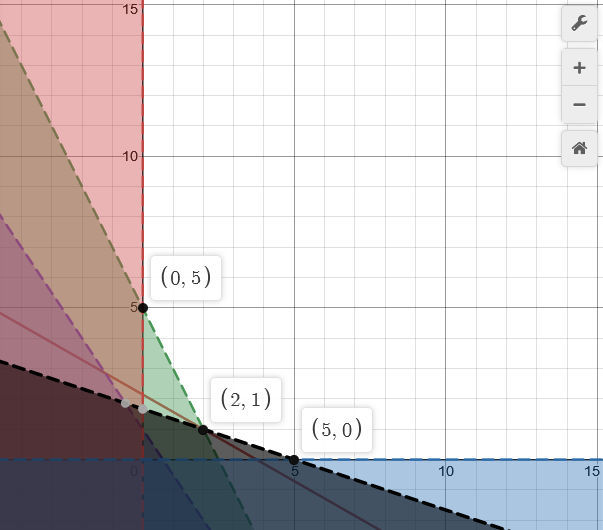
\includegraphics{1a.png}\\
    So we see that we have three points to check: $(0, 5) \ (2, 1) \ (5, 0)$. Using 
    algebra and these three points: 
    \begin{gather*}
        4(0) + 7(5) = 35\\
        4(2) + 7(1) = 15\\
        4(5) + 7(0) = 20
    \end{gather*}
    Thus, we find that the point $(2, 1)$ minimizes our function with subject to the 
    given restraints. 

    \item 
    \begin{enumerate}
        \item $x_1 + 5x_2 + 3x_3 + 7 x_4 + 5x_5$
        \item $
        \begin{bmatrix}
            48 \\ 
            45 \\
            26
        \end{bmatrix}
        $
    \end{enumerate}

    \item 
    \begin{gather*}
        \text{maximize} \ 5x_1 + 2x_2 + 5x_3\\
        \text{subject to} \ 2x_1 + 3x_2 + x_3 \leq 4\\
        x_1 + 2x_2 + 3x_3 \leq 7 \\
        x_1, x_2, x_3 \geq 0
    \end{gather*}
    Writing this problem in matrix-vector notation: 
    \begin{gather*}
        \text{maximize } z = 
        \begin{bmatrix}
            5 & 2 & 5
        \end{bmatrix}
        \begin{bmatrix}
            x_1 \\ x_2 \\ x_3
        \end{bmatrix}
        \\
        \text{subject to: }
        \begin{bmatrix}
            2 & 3 & 1\\
            1 & 2 & 3
        \end{bmatrix}
        \begin{bmatrix}
            x_1 \\ x_2 \\ x_3
        \end{bmatrix} 
        \leq 
        \begin{bmatrix}
            4 \\ 7
        \end{bmatrix}
        \\
        \begin{bmatrix}
            x_1\\ x_2\\ x_3 
        \end{bmatrix}
        \geq 
        \begin{bmatrix}
            0 \\ 0 \\ 0
        \end{bmatrix}
    \end{gather*}
\end{enumerate}

\end{document}